\documentclass[12pt]{article}

\usepackage{discrete}

\def\thetitle{Introduction to Graph Theory} % will be put in the center header on the first page only.
\def\lefthead{Math 228 Notes} % will be put in the left header
\def\righthead{\thetitle} % will be put in the right header



\begin{document}

\begin{activity}
In the time of Euler, in the town of K\"onigsberg in Prussia, there was a river containing two islands.  The islands were connected to the banks of the river by seven bridges (as seen below).  The bridges were very beautiful, and on their days off, townspeople would spend time walking over the bridges.  As time passed, a question arose: was it possible to plan a walk so that you cross each bridge once and only once?  Euler was able to answer this question.  Are you?

%\centerline{\includegraphics[width=5in]{images/7bridgescolor.png}}

\begin{center}
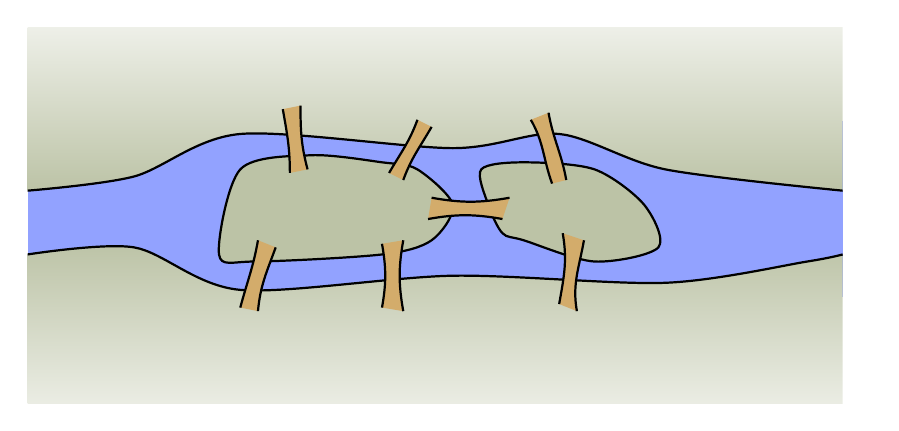
\begin{tikzpicture}[scale=0.9]
\definecolor{land}{HTML}{BCC3A6}
%\definecolor{land}{HTML}{FFFFFF}
\definecolor{water}{HTML}{92A2FF}
\definecolor{bridge}{HTML}{D3AC6B}
\clip (-6,-2.8) rectangle (5.9,2.5);
%River:
%\path[fill=water]plot[smooth] coordinates {(-6,-.7) (-6,.2) (-3,.9) (-2,1.2) (0,.8) (1,1) (3,.5) (6,.2)(6,-.8) (4.5, -1)  (2.8, -1.2) (.5, -1) (-2, -1.4) (-4.5, -.6) (-6,-.7)};
\fill[color=water] (-6,-1.3) rectangle (5.5,1.19);
%Islands:
\draw[thick, fill=land] plot[smooth cycle] coordinates {(0,0) (-.5, .5) (-1,.6) (-2, .7) (-3,.5) (-3.3, -.7) (-2.8, -.8) (-1,-.7) (-.3, -.5)};
\draw[thick, fill=land] plot[smooth cycle] coordinates {(.5,0) (.4,.5) (1,.6) (2,.5) (2.7,0) (2.9,-.6) (2,-.8) (1,-.5) (.7,-.4)};
%Banks:
\shade[bottom color=land, top color=white!90!land] plot[smooth] coordinates {(-6,.2) (-4.5,.4) (-3,1) (0,.8) (1.5,1) (3,.5) (5.5,.2)} -- plot coordinates {(5.5,3) (-6,3)};
\draw[thick] plot[smooth] coordinates {(-6,.2) (-4.5,.4) (-3,1) (0,.8) (1.5,1) (3,.5) (5.5,.2)};
\shade[top color=land, bottom color=white!75!land] plot[smooth] coordinates {(-6,-.7) (-4.5,-.6) (-3,-1.2) (0,-1) (3,-1.1) (5,-.8) (5.5,-.7)} -- plot coordinates {(5.5,-3) (-6,-3)};
\draw[thick] plot[smooth] coordinates {(-6,-.7) (-4.5,-.6) (-3,-1.2) (0,-1) (3,-1.1) (5,-.8) (5.5,-.7)};
%Bridges:
\path[fill=bridge] (-.3,.1) to[out=-10, in=190] (.8,.1) -- (.7, -.2) to[out=170, in=10] (-.35,-.2) -- cycle;
\draw[thick] (-.3,.1) to[out=-10, in=190] (.8,.1) (.7, -.2) to[out=170, in=10] (-.35,-.2);
\path[fill=bridge] (1.75,-1.5) to[out=100, in=260] (1.85,-.5) -- (1.55, -.4) to[out=280, in=80] (1.5,-1.4) -- cycle;
\draw[thick] (1.75,-1.5) to[out=100, in=260] (1.85,-.5) (1.55, -.4) to[out=280, in=80] (1.5,-1.4);

\path[fill=bridge] (1.6,.35) to[out=100, in=280] (1.35,1.3) -- (1.1, 1.2) to[out=300, in=110] (1.4,.3) -- cycle;
\draw[thick] (1.6,.35) to[out=100, in=280] (1.35,1.3) (1.1, 1.2) to[out=300, in=110] (1.4,.3);

\path[fill=bridge] (-.7,.35) to[out=70, in=240] (-.3,1.1) -- (-.5, 1.2) to[out=250, in=60] (-.9,.45) -- cycle;
\draw[thick] (-.7,.35) to[out=70, in=240] (-.3,1.1) (-.5, 1.2) to[out=250, in=60] (-.9,.45);

\path[fill=bridge] (-2.05,.5) to[out=105, in=270] (-2.15,1.4) -- (-2.4, 1.35) to[out=280, in=90] (-2.3,.45) -- cycle;
\draw[thick] (-2.05,.5) to[out=105, in=270] (-2.15,1.4) (-2.4, 1.35) to[out=280, in=90] (-2.3,.45);

\path[fill=bridge] (-2.75,-1.5) to[out=85, in=250] (-2.5,-.6) -- (-2.75, -.5) to[out=260, in=75] (-3,-1.45) -- cycle;
\draw[thick] (-2.75,-1.5) to[out=85, in=250] (-2.5,-.6) (-2.75, -.5) to[out=260, in=75] (-3,-1.45);

\path[fill=bridge] (-.7,-1.5) to[out=100, in=260] (-.7,-.5) -- (-1, -.55) to[out=280, in=80] (-1,-1.45) -- cycle;
\draw[thick] (-.7,-1.5) to[out=100, in=260] (-.7,-.5) (-1, -.55) to[out=280, in=80] (-1,-1.45);
%\path[shade, shading=radial, inner color=green!50!gray] (-7,-4) rectangle (7,4);
\end{tikzpicture}
\end{center}

%Try finding a path which uses each bridge exactly once.
\end{activity}
Graph Theory is a relatively new area of mathematics, first studied by the super famous mathematician Leonhard Euler in 1735.  Since then it has blossomed in to a powerful tool used in nearly every branch of science and is currently an active area of mathematics research.

The problem above, known as the \emph{Seven Bridges of K\"onigsberg}\index{K\"onigsberg}, is the problem that originally inspired graph theory.   Consider a ``different'' problem:  Below is a drawing of four dots connected by some lines.  Is it possible to trace over each line once and only once (without lifting up your pencil, starting and ending on a dot)?

\centerline{\begin{tikzpicture}[scale=0.9, yscale=.5]
 \draw (-1,-2) \v to [out=120, in=240] (-1,0) \v to [out=120, in=240] (-1,2) \v to [out=300, in=60] (-1,0) to [out=300, in=60] (-1,-2);
  \draw (1,0) \v -- (-1,2) (-1,0) -- (1,0) -- (-1,-2);
  \end{tikzpicture}}

There is an obvious connection between these two problems.  Any path in the dot and line drawing corresponds exactly to a path over the bridges of K\"onigsberg.

Pictures like the dot and line drawing are called {\em graphs}. %\footnote{Actually, since the picture here has dots connected by more than one line, it is called a \emph{multigraph}.}
Graphs are made up of a collection of dots called {\em vertices}\index{vertices} and lines connecting those dots called \emph{edges}\index{edges}.  When two vertices are connected by an edge, we say they are \emph{adjacent}\index{adjacent}.  The nice thing about looking at graphs instead of pictures of rivers, islands and bridges is that we now have a mathematical object to study:  a {\em set} containing of a set of vertices and a set of edges (in fact, we can take the set of edges to be a set of two element subsets from the set of vertices).  We have distilled the ``important'' parts of the bridge picture for the purposes of the problem.  It does not matter how big the islands are, what the bridges are made out of, if the river contains alligators, etc.  All that matters is which land masses are connected to which other land masses, and how many times.  This was the great insight that Euler had.

We will return to the question of finding paths through graphs later.  But first, here are a few other situations you can represent with graphs.

\begin{example}
  Al, Bob, Cam, Dan, and Euclid are all members of the social networking website {\em Facebook}.  The site allows members to be ``friends'' with each other.  It turns out that Al and Cam are friends, as are Bob and Dan.  Euclid is friends with everyone.  Represent this situation with a graph.
  \begin{solution}
    Each person will be represented by a vertex and each friendship will be represented by an edge.  That is, there will be an edge between two vertices if and only if the people represented by those vertices are friends.  We get the following graph:

    \begin{center}
      \begin{tikzpicture}[scale=0.7]
        \draw(-1, 0) \vl{C} -- (0,1) \vb{E} -- (-1,2) \vl{A} -- (-1,0)(1,0) \vr{D} -- (0,1)  -- (1,2) \vr{B} -- (1,0);
      \end{tikzpicture}
    \end{center}
  \end{solution}

\end{example}


\begin{example}
  Each of three houses must be connected to each of three utilities.  Is it possible to do this without any of the utility lines crossing?
  \begin{solution}
    We will answer this question later.  For now, notice how we would ask this question in the context of graph theory.  We are really asking whether it is possible to redraw the graph below without any edges crossing (except at vertices).

    \begin{center}
      \begin{tikzpicture}[yscale=.8]
        \draw (-1,1) \v -- (-1,0)\v  -- (0,1) \v -- (0,0) \v -- (1,1) \v -- (1,0) \v -- (0,1) -- (-1,0) -- (1,1) (1,0) -- (-1,1) -- (0,0);
      \end{tikzpicture}
    \end{center}

  \end{solution}

\end{example}

\section{Basics}


\begin{activity}

\begin{questions}
\question Which (if any) of the graphs below are the same?


\begin{tikzpicture}
\coordinate (A) at (-1,0);
\coordinate (B) at (0,0);
\coordinate (C) at (1,0);
\coordinate (D) at (-.5,1);
\coordinate (E) at (.5,1);

\draw  (A) -- (D) -- (B) -- (E) -- (C) -- (D)  (A) -- (E);
\foreach \x in {(A), (B), (C), (D), (E)}{
	\fill \x \v;
}
\end{tikzpicture}
\hfill
\begin{tikzpicture}
\coordinate (A) at (90+360/5:1);
\coordinate (B) at (90+2*360/5:1);
\coordinate (C) at (90+3*360/5:1);
\coordinate (D) at (90+4*360/5:1);
\coordinate (E) at (90:1);

\draw  (A) -- (B) -- (C) -- (D) -- (E) -- (A);
\foreach \x in {(A), (B), (C), (D), (E)}{
	\fill \x \v;
}
\end{tikzpicture}
\hfill
\begin{tikzpicture}
\coordinate (A) at (-1,0);
\coordinate (B) at (0,1);
\coordinate (C) at (0,0);
\coordinate (D) at (0,-1);
\coordinate (E) at (1,0);

\draw  (A) -- (B) -- (E) -- (C) -- (A) -- (D) -- (E);
\foreach \x in {(A), (B), (C), (D), (E)}{
	\fill \x \v;
}
\end{tikzpicture}
\hfill
\begin{tikzpicture}
\coordinate (A) at (90+360/5:1);
\coordinate (B) at (90+2*360/5:1);
\coordinate (C) at (90+3*360/5:1);
\coordinate (D) at (90+4*360/5:1);
\coordinate (E) at (90:1);

\draw  (A) -- (C) -- (E) -- (B) -- (D) -- (A);
\foreach \x in {(A), (B), (C), (D), (E)}{
	\fill \x \v;
}
\end{tikzpicture}
\hfill
\begin{tikzpicture}
\coordinate (A) at (-1,0);
\coordinate (B) at (0,1);
\coordinate (C) at (0,0);
\coordinate (D) at (0,-1);
\coordinate (E) at (1,0);

\draw  (A) -- (C) -- (B) (D) -- (C) -- (E);
\foreach \x in {(A), (B), (C), (D), (E)}{
	\fill \x \v;
}
\end{tikzpicture}
\hfill
~



\question The graphs above are unlabeled.  Usually we think of a graph as having a specific set of vertices.  Which (if any) of the graphs below are the same?

\begin{tikzpicture}
\coordinate (A) at (-1,0);
\coordinate (B) at (-1, 1);
\coordinate (C) at (0,0);
\coordinate (D) at (0,1);
\coordinate (E) at (1,0);
\coordinate (F) at (1,1);

\draw  (A) node[below] {$a$} -- (B) node[above] {$b$} -- (C) node[below] {$c$} -- (D) node[above] {$d$} -- (E) node[below] {$e$} -- (F) node[above] {$f$} -- (C) (A) -- (D);
\foreach \x in {(A), (B), (C), (D), (E), (F)}{
	\fill \x \v;
}
\end{tikzpicture}
\hfill
\begin{tikzpicture}
\coordinate (A) at (-1,0);
\coordinate (B) at (-1, 1);
\coordinate (C) at (0,1);
\coordinate (D) at (0,0);
\coordinate (E) at (1,0);
\coordinate (F) at (1,1);

\draw (A) node[below] {$a$} -- (B) node[above] {$b$} -- (C) node[above] {$c$} -- (D) node[below] {$d$} -- (E) node[below] {$e$} -- (F) node[above] {$f$} -- (C) (A) -- (D);
\foreach \x in {(A), (B), (C), (D), (E), (F)}{
	\fill \x \v;
}
\end{tikzpicture}
\hfill
\begin{tikzpicture}
\coordinate (A) at (-1,0);
\coordinate (B) at (-1, 1);
\coordinate (C) at (0,0);
\coordinate (D) at (0,1);
\coordinate (E) at (1,0);
\coordinate (F) at (1,1);

\draw (A) node[below] {$a$} -- (B) node[above] {$c$} -- (C) node[below] {$e$} -- (D) node[above] {$b$} -- (E) node[below] {$d$} -- (F) node[above] {$f$} -- (C) (A) -- (D);
\foreach \x in {(A), (B), (C), (D), (E), (F)}{
	\fill \x \v;
}
\end{tikzpicture}
\hfill
\begin{tikzpicture}
\coordinate (A) at (-1,0);
\coordinate (B) at (-1, 1);
\coordinate (C) at (0,1);
\coordinate (D) at (0,0);
\coordinate (E) at (1,0);
\coordinate (F) at (1,1);

\draw (A) node[below] {$v_6$} -- (B) node[above] {$v_1$} -- (C) node[above] {$v_2$} -- (D) node[below] {$v_5$} -- (E) node[below] {$v_4$} -- (F) node[above] {$v_3$} -- (C) (A) -- (D);
\foreach \x in {(A), (B), (C), (D), (E), (F)}{
	\fill \x \v;
}
\end{tikzpicture}



\question Actually, all the graphs we have seen above are just {\em drawings} of graphs.  A graph is really an abstract mathematical object consisting of two sets $V$ and $E$ where $E$ is a set of 2-element subsets of $V$.

Are the graphs below the same or different?
\begin{itemize}
\item[Graph 1:] $V = \{a, b, c, d, e\}$, $E = \{\{a,b\}, \{a, c\}, \{a,d\}, \{a,e\}, \{b,c\}, \{d,e\}\}$.


\item[Graph 2:] $V = \{v_1, v_2, v_3, v_4, v_5\}$,\\ $E = \{\{v_1, v_3\}, \{v_1, v_5\}, \{v_2, v_4\}, \{v_2, v_5\}, \{v_3, v_5\}, \{v_4, v_5\}\}$.

\end{itemize}

\end{questions}

\end{activity}


While we almost always think of graphs as pictures, these are really just visual representations of mathematical objects.  In fact, a graph is simply a set of vertices some pairs of which are ``related'' by an edge.  For example, we can describe a particular graph like this: the vertices are the letters $\{a,b,c,d\}$ and the edges are the pairs \[\{\{a,b\}, \{a,c\}, \{b,c\}, \{b,d\}, \{c,d\}\}.\]  %Technically the edges are 2-elements subsets of the set of vertices, so we should write $(a,b)$ as $\{a,b\}$ but we use parentheses to ease reading.
We could have described the graph in words as follows: we have four vertices, $a$, $b$, $c$, and $d$, and $a$ is adjacent to $b$ and $c$, $b$ is adjacent to both $c$ and $d$, and $c$ is also adjacent to $d$.  One way to draw this graph is this:
\begin{center}
  \begin{tikzpicture}[scale=0.7]
    \draw  (-1,1) \vl{$a$} -- (1,1) \vr{$b$} (-1,1) -- (-1,-1) \vl{$c$} -- (1,-1) \vr{$d$} -- (1,1) -- (-1,-1);
  \end{tikzpicture}
\end{center}

However we could also have drawn the graph differently.  For example either of these:

\begin{center}
  \begin{tikzpicture}[scale=0.7]
    \draw  (-1,1) \vl{$a$} -- (1,-1) \vr{$b$} (-1,1) -- (-1,-1) \vl{$c$} -- (1,1) \vr{$d$} -- (1,-1) -- (-1,-1);
  \end{tikzpicture}
  \hspace{1in}
    \begin{tikzpicture}[scale=0.7]
    \draw  (-1.5,0) \vb{$a$} -- (-.5,0) \vb{$b$} (-1.5,0) .. controls (-.5,1) .. (.5,0) \vb{$c$} -- (1.5,0) \vb{$d$} .. controls (.5,1) .. (-.5,0) -- (.5,0);
  \end{tikzpicture}
\end{center}

We should be careful about what it means for two graphs to be ``the same.''  Remember, as mathematical objects, graphs are just sets.  Two sets are equal if they have the exact same members.  However, even if two graphs are not \emph{equal}, they might be \emph{basically} the same.  Graphs that are basically the same (but perhaps not equal) are called \emph{isomorphic}.  We will give a precise definition of this term after a quick example:

\begin{example}
Consider the graphs:\\ $G_1 = \{V_1, E_1\}$ where $V_1 = \{a, b, c\}$ and $E_1 = \{\{a,b\}, \{a,c\}, \{b,c\}\}$; \\$G_2 = \{V_2, E_2\}$ where $V_2 = \{u,v,w\}$ and $E_2 = \{\{u,v\}, \{u,w\}, \{v,w\}\}$. \\
Are these graphs the same?

\begin{solution}
The two graphs are NOT equal.  It is enough to notice that $V_1 \ne V_2$ since $a \in V_1$ but $a \notin V_2$.  However, both of these graphs consist of three vertices with edges connecting every pair of vertices.  We can draw them as follows:

\begin{center}
\begin{tikzpicture}
\draw  (90:1) \va{$a$} -- (210:1) \vl{$b$} -- (-30:1) \vr{$c$} -- (90:1);
\end{tikzpicture}
\qquad
\begin{tikzpicture}
\draw  (90:1) \va{$u$} -- (210:1) \vl{$v$} -- (-30:1) \vr{$w$} -- (90:1);
\end{tikzpicture}
\end{center}
Clearly we want to say these graphs are basically the same, so while they are not equal, they will be \emph{isomorphic}.  The reason is we can rename the vertices of one graph and get the second graph as the result.
\end{solution}
\end{example}

Intuitively, graphs are \emph{isomorphic}\index{isomorphic} if they are basically the same, or better yet, if they are the same except for the names of the vertices.  To make the concept of renaming vertices precise, we give the following definitions:


\begin{defbox}{Isomorphic Graphs\index{isomorphic}}
An \emph{isomorphism}\index{isomorphism} between two graphs $G_1$ and $G_2$ is a bijection $f:V_1 \to V_2$ between the vertices of the graphs such that if $\{a,b\}$ is an edge in $G_1$ then $\{f(a), f(b)\}$ is an edge in $G_2$.

Two graphs are \emph{isomorphic} if there is an isomorphism between them.  In this case we write $G_1 \gls{isom} G_2$.
\end{defbox}

An isomorphism is simply a function which renames the vertices.  It must be a bijection so every vertex gets a new name.  These newly named vertices must be connected by edges precisely if they were connected by edges with their old names.

\begin{example}
Decide whether the graphs $G_1 = \{V_1, E_1\}$ and $G_2 = \{V_2, E_2\}$ are equal or isomorphic.

$V_1 = \{a,b,c,d\}$, $E_1 = \{\{a,b\}, \{a,c\}, \{a,d\}, \{c,d\}\}$

$V_2 = \{a,b,c,d\}$, $E_2 = \{\{a,b\}, \{a,c\}, \{b,c\}, \{c,d\}\}$

\begin{solution}
The graphs are NOT equal, since $\{a,d\} \in E_1$ but $\{a,d\} \notin E_2$.  However, since both graphs contain the same number of vertices and same number of edges, they \emph{might} be isomorphic (this is not enough in most cases, but it is a good start).

We can try to build an isomorphism.  How about we say $f(a) = b$, $f(b) = c$, $f(c) = d$ and $f(d) = a$.  This is definitely a bijection, but to make sure that the function is an isomorphism, we must make sure it \emph{respects the edge relation}.  In $G_1$, vertices $a$ and $b$ are connected by an edge.  In $G_2$, $f(a) = b$ and $f(b) = c$ are connected by an edge.  So far, so good, but we must check the other three edges.  The edges $\{a,c\}$ in $G_1$ corresponds to $\{f(a), f(c)\} = \{b,d\}$, but here we have a problem.  There is no edge between $b$ and $d$ in $G_2$.  Thus $f$ is NOT an isomorphism.

Not all hope is lost, however.  Just because $f$ is not an isomorphism does not mean that there is no isomorphism at all.  We can try again.  At this point it might be helpful to draw the graphs to see how they should match up.  Alternatively, notice that in $G_1$, the vertex $a$ is adjacent to every other vertex.  In $G_2$, there is also a vertex with this property: $c$.  So build the bijection $g:V_1 \to V_2$ by defining $g(a) = c$ to start with.  Next, where should we send $b$?  In $G_1$, the vertex $b$ is only adjacent to vertex $a$.  There is exactly one vertex like this in $G_2$, namely $d$.  So let $g(b) = d$.  As for the last two, in this example, we have a free choice: let $g(c) = b$ and $g(d) = a$ (switching these would be fine as well).

We should check that this really is an isomorphism.  It is definitely a bijection.  We must make sure that the edges are respected.  The four edges in $G_1$ are
\[\{a,b\}, \{a,c\}, \{a,d\}, \{c,d\}\]
Under the proposed isomorphism these become
\[\{g(a), g(b)\}, \{g(a), g(c)\}, \{g(a), g(d)\}, \{g(c), g(d)\}\]
\[ \{c,d\}, \{c,b\}, \{c,a\}, \{b,a\}\]
which are precisely the edges in $G_2$.  Thus $g$ is an isomorphism, so $G_1 \cong G_2$

\end{solution}
\end{example}

Sometimes we will talk about a graph with a special name (like $K_n$ or the \emph{Peterson graph}) or perhaps draw a graph without any labels.  In this case we are really referring to \emph{all} graphs isomorphic to any copy of that particular graph.  A collection of isomorphic graphs is often called an \emph{isomorphism class}\index{isomorphism class}.\footnote{This is not unlike geometry, where we might have more than one copy of a particular triangle.  There instead of \emph{isomorphic} we say \emph{congruent}.}

Back to some basic graph theory definitions.  Notice that the graphs above have the property that no pair of vertices is connected more than once, and no vertex is connected to itself.  Graphs like these are sometimes called {\em simple}, although we will just call them {\em graphs}.  This is because our definition for a graph says that the edges form a set of 2-element subsets of the vertices.  Remember that it doesn't make sense to say a set contains an element more than once.  So no pair of vertices can be connected by an edge more than once.  And since each edge must be a set containing two vertices, we cannot have a single vertex connected to itself by an edge.

That said, there are times we want to consider double (or more) edges and single edge loops.  For example, the ``graph'' we drew for the Bridges of K\"onigsberg problem had double edges because there really are two bridges connecting a particular island to the near shore.  We will call these objects {\em multigraphs}\index{multigraph}.  This is a good name: a \emph{multiset} is a set in which we are allowed to include a single element multiple times.

The graphs above are also {\em connected}\index{connected}: you can get from any vertex to any other vertex by following some path of edges.  A graph that is not connected can be thought of as two separate graphs drawn close together.  Unless otherwise stated, we will assume all our graphs are connected.

Vertices in a graph do not always have edges between them.  If we add all possible edges, then the resulting graph is called {\em complete}\index{complete graph}.  That is, a graph is complete if every pair of vertices is connected by an edge.  Since a graph is determined completely by which vertices are adjacent to which other vertices, there is only one complete graph with a given number of vertices.  We give these a special name: \gls{Kn} is the complete graph on $n$ vertices.

Each vertex in $K_n$ is adjacent to $n-1$ other vertices.  We call the number of edges emanating from a given vertex the {\em degree} of that vertex.  So every vertex in $K_n$ has degree $n-1$.  How many edges does $K_n$ have?  One might think the answer should be $n(n-1)$, since we count $n-1$ edges $n$ times (once for each vertex).  However, each edge is incident to 2 vertices, so we counted every edge exactly twice.  Thus there are $n(n-1)/2$ edges in $K_n$.
Alternatively, we can say there are ${n \choose 2}$ edges, since to draw an edge we must choose 2 of the $n$ vertices.

In general, if we know the degrees of all the vertices in a graph we can find the number of edges.  The sum of the degrees of all vertices will always be \underline{twice} the number of edges, since each edge adds to the degree of two vertices.  Notice this means that the sum of the degrees of all vertices in any graph must be even!

\begin{example}
  At a recent math seminar, 9 mathematicians greeted each other by shaking hands.  Is it possible that each mathematician shook hands with exactly 7 people at the seminar?
  \begin{solution}
    It seems like this should be possible.  Each mathematician chooses one person to not shake hands with.  But this cannot happen.  We are asking whether a graph with 9 vertices can have each vertex have degree 7.  If such a graph existed, the sum of the degrees of the vertices would be $9\cdot 7 = 63$.  This would be twice the number of edges (handshakes) resulting in a graph with $31.5$ edges.  That is impossible.  Thus at least one (in fact an odd number) of the mathematicians must have shaken hands with an {\em even} number of people at the seminar.
  \end{solution}

\end{example}

One final definition: we say a graph is {\em bipartite}\index{bipartite} if the vertices can be divided into two sets, $A$ and $B$, with no two vertices in $A$ adjacent and no two vertices in $B$ adjacent.  The vertices in $A$ can be adjacent to some or all of the vertices in $B$.  If each vertex in $A$ is adjacent to all the vertices in $B$, then the graph is a {\em complete bipartite graph}, and gets a special name: $K_{m,n}$, where $|A| = m$ and $|B| = n$.  The graph in the houses and utilities puzzle is $K_{3,3}$.

\begin{defbox}{Named Graphs}
  Some graphs are used more than others, and get special names.
  \begin{itemize}
    \item[] \gls{Kn}: the complete graph on $n$ vertices.
    \item[] \gls{Kmn}: the complete bipartite graph with sets of $m$ and $n$ vertices.
    \item[] \gls{Cn}: the cycle graph on $n$ vertices, just one big loop.
    \item[] \gls{Pn}: the path graph on $n$ vertices, just one long path.
  \end{itemize}
 % Here are some typical examples:

\def\sb{.6}
\begin{center}
\hfill
\begin{tikzpicture}[scale=\sb+.05]
  \path (0,.9) +(18:1) coordinate (a);
  \path (0,.9) +(90:1) coordinate (b);
  \path (0,.9) +(162:1) coordinate (c);
  \path (0,.9) +(234:1) coordinate (d);
  \path (0,.9) +(306:1) coordinate (e);
  \draw  (a) \v -- (b) \v -- (c) \v -- (d) \v -- (e) \v -- (a) -- (c) -- (e) -- (b) -- (d) -- (a);
  \draw (0,-.5) node[below]{\large $K_5$};
\end{tikzpicture}
\hfill
\begin{tikzpicture}[scale=\sb, xscale=1.5]
 \draw  (-1, 0) \v -- (-.5,2) \v -- (0,0) \v -- (.5, 2) \v -- (1,0) \v -- (-.5,2) (.5,2) -- (-1,0);
 \draw (0,-.5) node[below]{\large $K_{2,3}$};
  \end{tikzpicture}
\hfill
\begin{tikzpicture}[scale=\sb]
  \draw  (0:1) \v -- (60:1) \v -- (120:1) \v -- (180:1) \v -- (240:1) \v -- (300:1) \v -- cycle;
  \draw (270:1.5) node[below]{\large $C_6$};
\end{tikzpicture}
\hfill
\begin{tikzpicture}[scale=\sb]
  \draw  (-2,0) \v -- (-1,.5) \v -- (0,0) \v -- (1,.75) \v -- (.5,1.5) \v -- (2,2) \v;
  \draw (0,-.5) node[below]{\large $P_6$};
\end{tikzpicture}
\hfill
~
\end{center}
\end{defbox}

\newpage

\begin{defbox}{Graph Theory Definitions}

\noindent\textbf{Graph}\index{graph}: A collection of {\em vertices}, some of which are connected by {\em edges}.  More precisely, a pair of sets $V$ and $E$ where $V$ is a set of vertices and $E$ is a set of 2-element subsets of $V$.
\vskip 1ex
\noindent \textbf{Adjacent}\index{adjacent}: Two vertices are {\em adjacent} if they are connected by an edge.  Two edges are {\em adjacent} if they share a vertex.
\vskip 1ex
\noindent \textbf{Bipartite graph}\index{bipartite}: A graph for which it is possible to divide the vertices into two disjoint sets such that there are no edges between any two vertices in the same set.
\vskip 1ex
\noindent\textbf{Complete bipartite graph}: A bipartite graph for which every vertex in the first set is adjacent to every vertex in the second set.
\vskip 1ex
\noindent\textbf{Complete graph}\index{complete graph}: A graph in which every pair of vertices is adjacent.
\vskip 1ex
\noindent\textbf{Connected}\index{connected}: A graph is {\em connected} if there is a path from any vertex to any other vertex.
\vskip 1ex
\noindent \textbf{Chromatic number}\index{chromatic number}: The minimum number of colors required in a proper vertex coloring of the graph.
\vskip 1ex
\noindent\textbf{Cycle}\index{cycle}: A path (see below) that starts and stops at the same vertex, but contains no other repeated vertices.
\vskip 1ex
\noindent \textbf{Degree of a vertex}\index{degree}: The number of edges incident to a vertex.
\vskip 1ex
\noindent \textbf{Euler path}: A path which uses each edge exactly once.
\vskip 1ex
\noindent \textbf{Euler circuit}\index{Euler path}: An Euler path which starts and stops at the same vertex.
\vskip 1ex
\noindent\textbf{Multigraph}\index{multigraph}: A {\em multigraph} is just like a graph but can contain multiple edges between two vertices as well as single edge loops (that is an edge from a vertex to itself).
\vskip 1ex
\noindent \textbf{Path}\index{path}: A sequence of vertices such that consecutive vertices (in the sequence) are adjacent (in the graph).  A path in which no vertex is repeated is called {\em simple}.
\vskip 1ex
\noindent \textbf{Planar}\index{planar}: A graph which can be drawn (in the plane) without any edges crossing.
\vskip 1ex
 \noindent\textbf{Subgraph}\index{subgraph}: We say that $H$ is a \emph{subgraph} of $G$ if every vertex and edge of $H$ is also a vertex or edge of $G$.  We say $H$ is an {\em induced} subgraph of $G$ if every vertex of $H$ is a vertex of $G$ and each pair of vertices in $H$ are adjacent in $H$ if and only if they are adjacent in $G$.
\vskip 1ex
\noindent \textbf{Tree}\index{tree}: A (connected) graph with no cycles.  (A non-connected graph with no cycles is called a {\em forest}.)  The vertices in a tree with degree 1 are called {\em leaves}.
\vskip 1ex
\noindent \textbf{Vertex coloring}\index{vertex coloring}: An assignment of colors to each of the vertices of a graph. A vertex coloring is {\em proper} if adjacent vertices are always colored differently.
\end{defbox}
\newpage

\end{document}
